\section{Materials and Methods}
\subsection{Experimental Setup}
The energetic incident protons were generated using a Van de Graff accelerator as shown in Figures \ref{fig_setup1}, \ref{fig_setup2} and \ref{fig_setup3}. The variety of incoming particles were limited by the source, which was a flask of hydrogen gas connected to the accelerator tank. The flask was not changed, and thus this experiment only concerns the ions $\mathrm{H^+}$ and $\mathrm{{H^2}^+}$, in particular protons. The accelerator ionized a hydrogen gas which could escape in a narrow beam. The particles were accelerated to an energy up to 400 keV controllable on the accelerator. The particles entered a big electromagnet which generates a magnetic field that controls the angle of deflection of the beam. By adjusting the field one could control which particles, depending on the mass and charge, could enter the beamline and thus interact with the target. 
The beam position may be corrected by adjusting four electrostatic plates, two vertical parallel and two horizontal parallel, before entering the scattering chamber.

From the beamline the particles were directed toward a chosen target material, where they got scattered on atomic nuclei of the target. A detector was placed at a movable position around the target, such that scattering angles up 160 degrees could be measured. 
The detector was coupled to a digitizer with a time resolution of xx s and  connected to a computer. During measurements the digitizer started a clock inside it. When the detector was hit by a particle, the digitizer translated the measured energy into a digital number and sent the number and the corresponding time stamp to the computer. 
The program Mc2Analyzer was used to handle the data. The digital number is an arbitrary number called a channel number. It is translatable to the actual energy by a linear factor plus an offset. In order to convert these channel numbers to correct energies of the scattered particles a calibration was done.

\subsection{Calibration}

The measured energy of a scattered particle is given as a digital output called a channel number. A calibration is necessary to convert these channel numbers to the actual particle scattering energies. Assuming a linear relationship between the energy and the channel number the energy can be found as 
\begin{equation}
E = \alpha(k - k_0),
\end{equation}
where $k$ is the channel and $k_0$ and $\alpha$ are constants. The constants in the relation is determined by varying the incoming energy and writing down the corresponding values of energy and channel number. The constants are determined from a linear fit of the energies as function of channel numbers.
With the Van de Graff accelerator the magnetic field can be adjusted to deflect either $\mathrm{H^+}$ or $\mathrm{{H_2}^+}$ into the beamline. For each of these a data point of energy related to channel number can be found. 
By considering energy and momentum conservation for elastic scattering in two dimensions the energy of the scattered particles $E_f$ can be found from the incident proton energy and the scattering angle as: 
\begin{equation}
E_f = \left( \frac{m_p \cos\theta + \sqrt{{m_t}^2 - {m_p}^2 \sin^2\theta}}{m_p+m_t} \right)^2 E_i,
\end{equation}
where $E_i$ is the energy of the incident beam particles, $m_p$ and $m_t$ are the masses of the incident protons and the target particles, respectively, and $\theta$ is the angle between the direct outgoing non-scattered beam and the scattered particles - also called the scattering angle.

Unfortunately, this only give two data points one from $\mathrm{H^+}$ and one from $\mathrm{{H_2}^+}$. The incline from the linear fit to these data points is still useful. However, another method is used to determine the zero-amplitude constant $k_0$. Different energies are generated using a pulse generator by changing the amplitude (corresponding to a change of resistance). For each fixed amplitude, a normal distribution of counts around a certain mean channel is obtained. The mean channel (also called the centroid) is determined from a Gaussian fit to the distribution. 

TABLE WITH CORRESPONDING VALUES OF AMPLITUDE AND MEAN CHANNEL (AND THEIR UNCERTAINTIES)!

FIGURE WITH AN EXAMPLE OF A GAUSSIAN FIT.

Figure X shows the count distribution as function of channels for the amplitude X fitted with gaussian function. The data clearly follows a gaussian distribution and the data points are, within uncertainty, well described by a gaussian distribution. 

From the fit the coefficient $k_0$ is .... 


\subsection{Targets}
The targets of interest in this experiment was a thin gold coated carbon plate. The gold coating was about one tenth of the carbon thickness. The thickness of the carbon plate have previously been determined as 250Å, and the thickness of the gold coating as 25Å.\footnotemark \footnotetext{The estimated thickness of each target available have been determined by the previous users of the experimental setup and written down on the whiteboard next to the setup.} 
The target was placed in holder, which contains several other targets. The height of the holder was fixed, though it was not investigated whether the marked height was optimal in relation to the beam position.
When measuring proton scattering at different angles, the blind angles of the target holder may cause a problem. In order to avoid the targets "blind-spots", the target was turned at an angle following the detector while still avoiding the incoming proton beam to end up in a blind angle. The blind angles  
  
der er en blinde vinkel omkring 30 grader og det er derfor en god ide at dreje target sammen med detektoren - dog ikke 90 grader, da vi så kun rammer target holderen.



%\begin{table}[h]
%\centering
%\caption{\sl De maalte data for kalibreringen af....}
%\begin{tabular}{l D{.}{,}{5.0} *{2}{ D{.}{,}{10.0} @{$\pm$} D{.}{,}{2.0} } %D{.}{,}{3.0}}
%\toprule
% \multicolumn{1}{c}{Target} & \multicolumn{2}{c}{Thickness (Å)} & %\multicolumn{2}{c}{Area density} \\
%\midrule
%LiF/C  &  ?  &  ? & 0.5 \\
%B/C  &  ?  &  ?  \\
%AL  &  ?  &  ?  \\
%Au/C  &  ?  &  ?  \\
%\bottomrule
%\end{tabular}
%\label{tbl:eksempel}
%\end{table}




\begin{figure}[h]
\centering
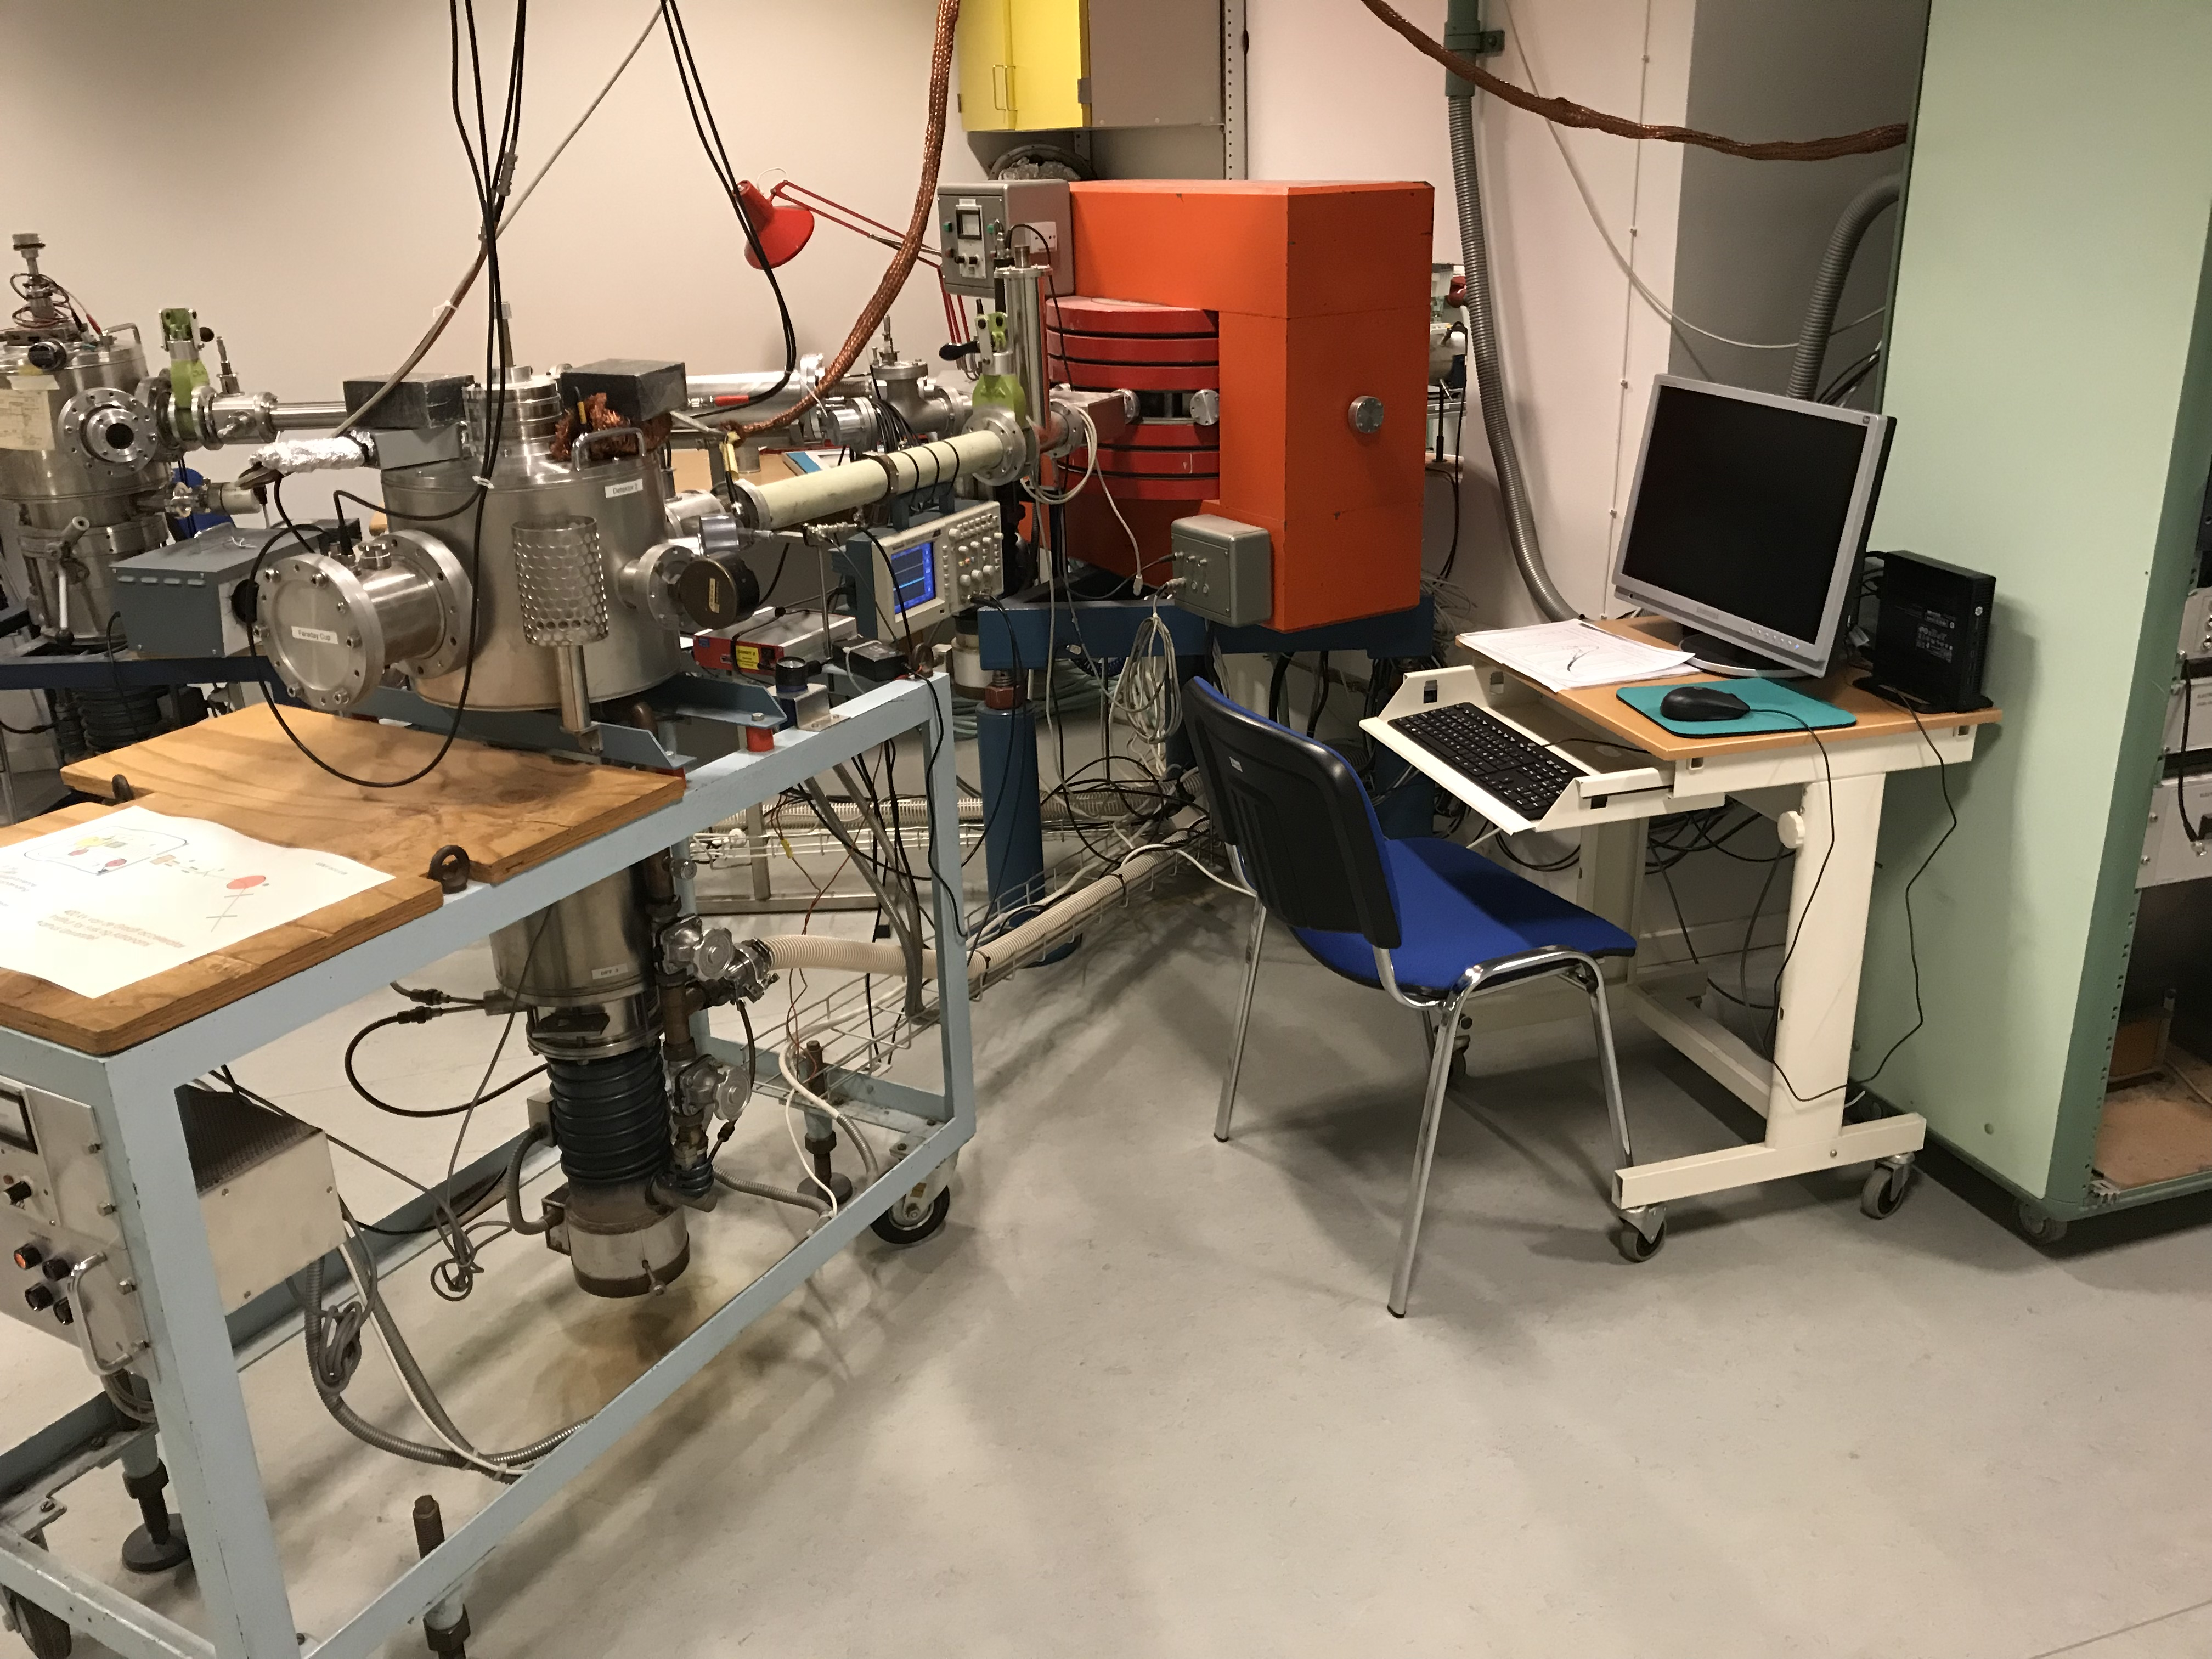
\includegraphics[width=0.5\textwidth]{setup1}
\caption{Experimental setup 1: The detector and a computer for the data
analysis.}
\label{fig_setup1}
\end{figure}

\begin{figure}[h]
\centering
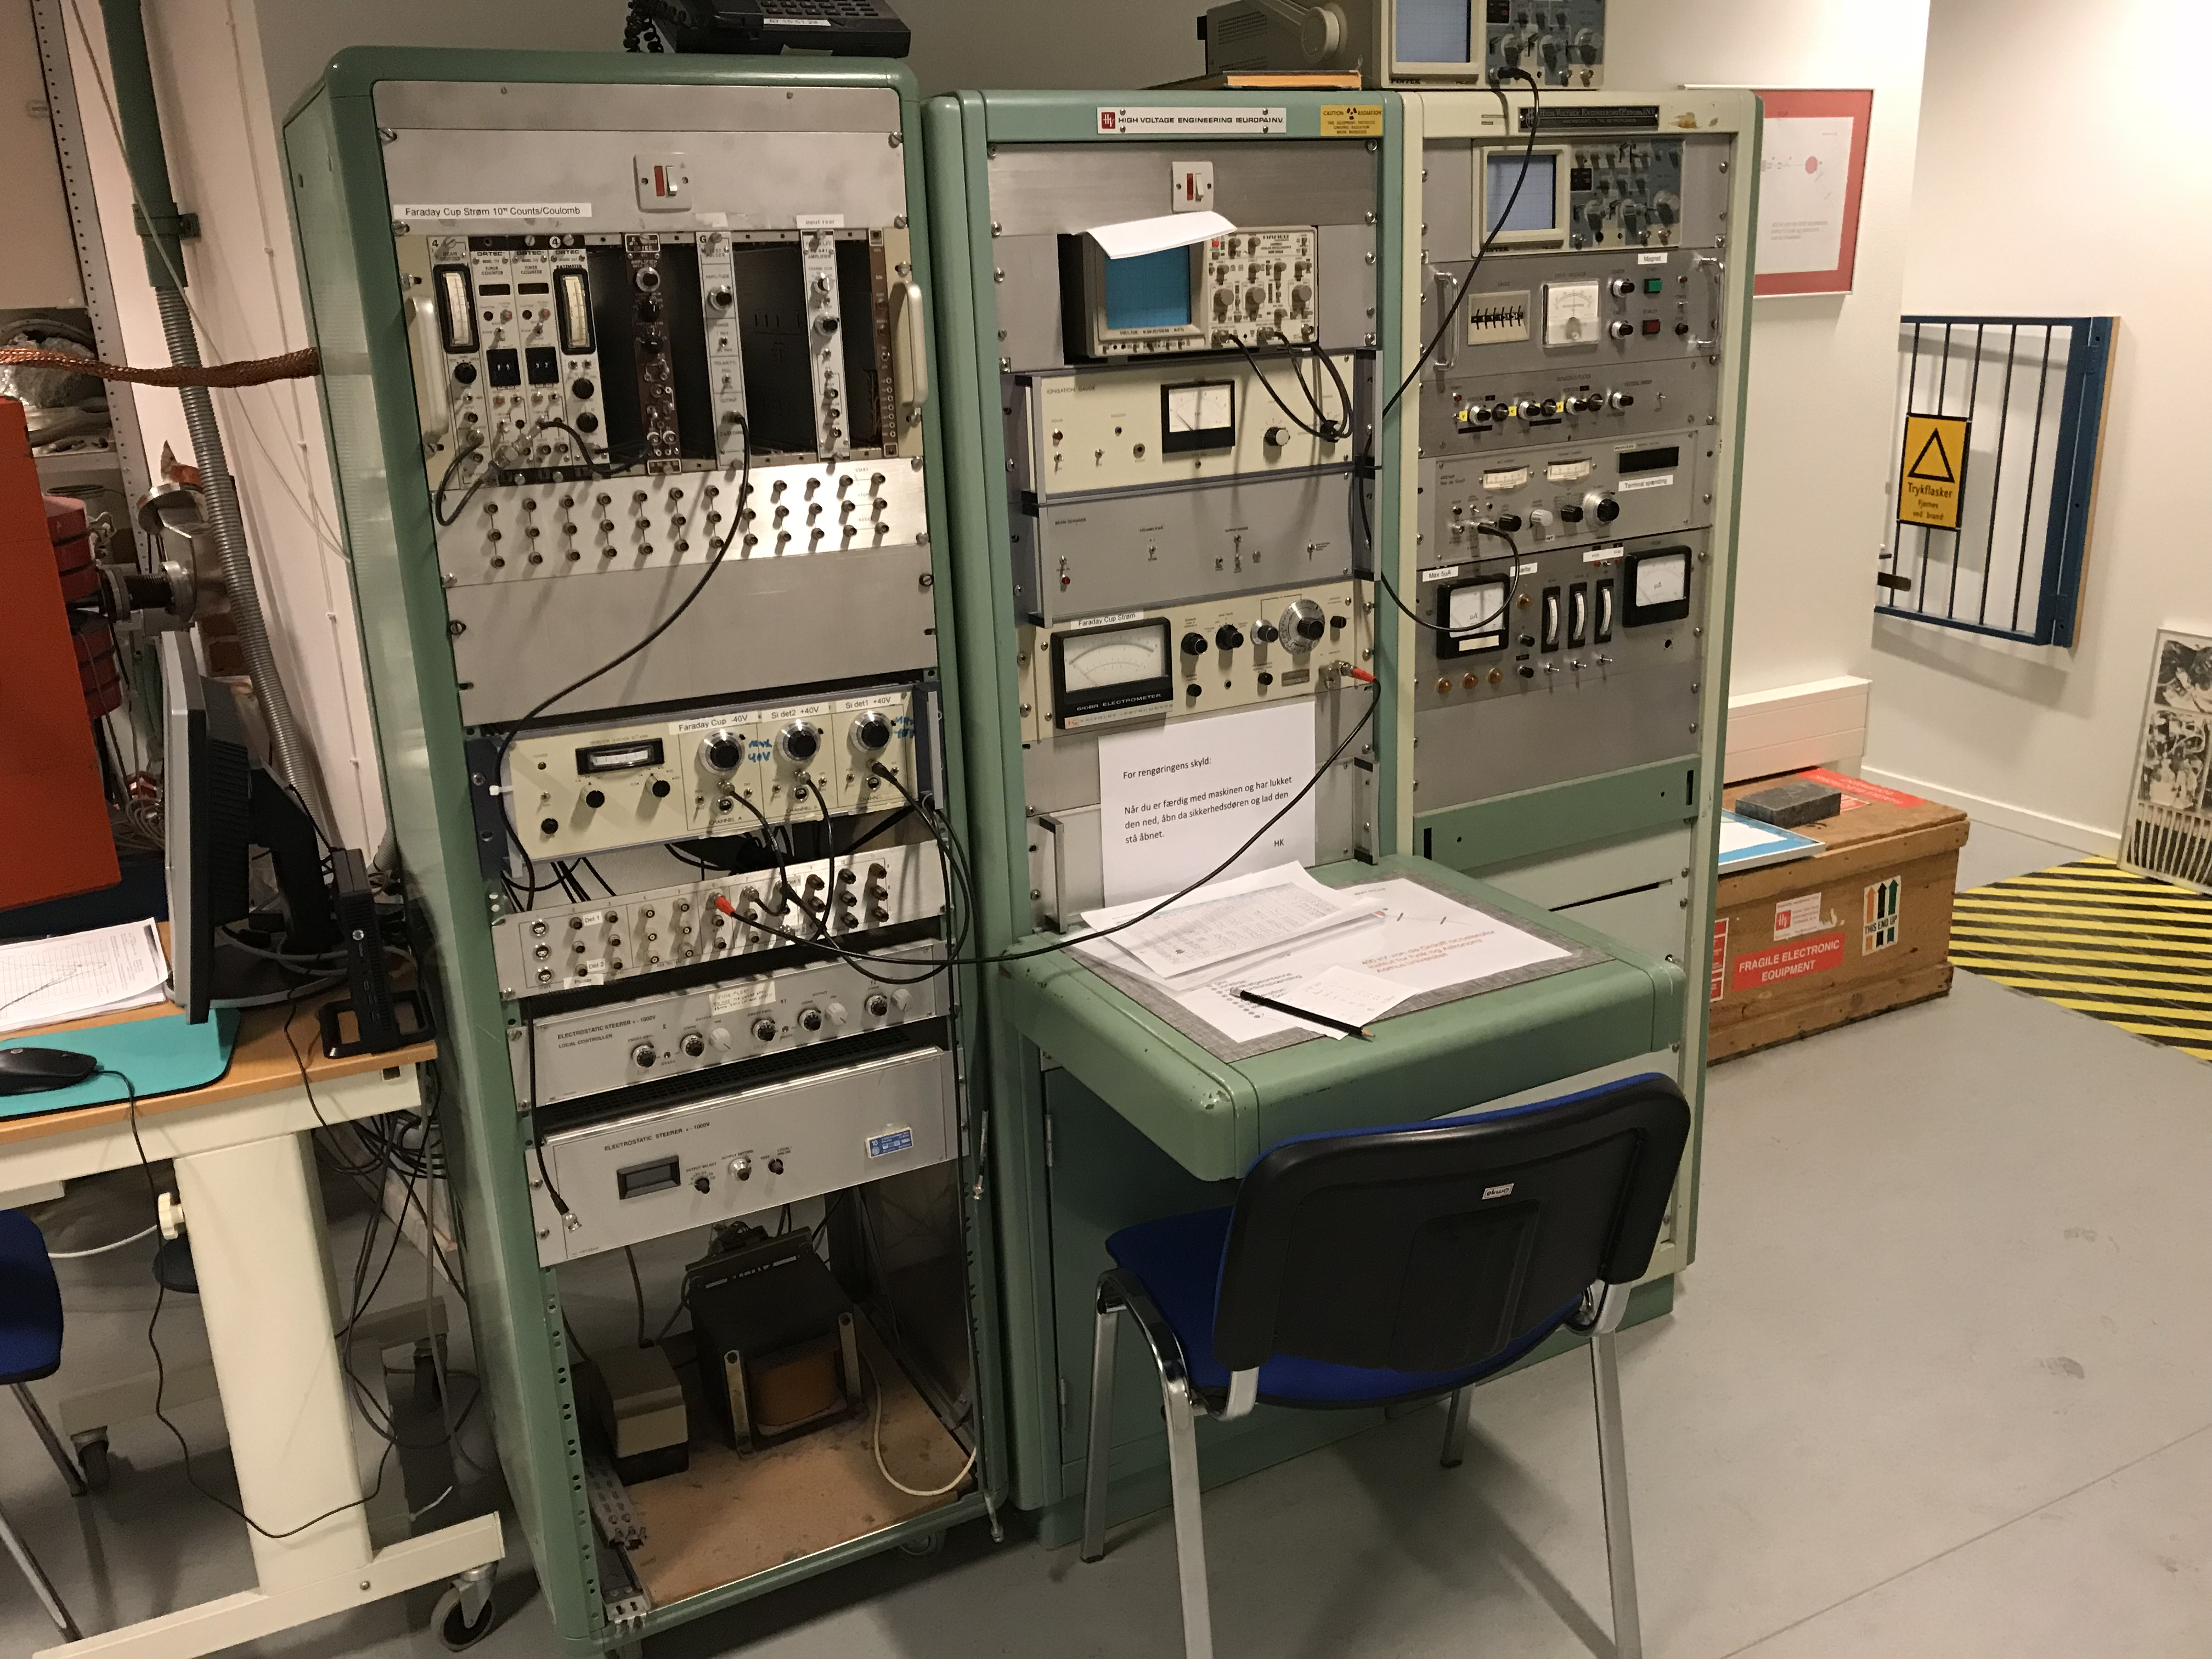
\includegraphics[width=0.5\textwidth]{setup2}
\caption{Experimental setup 2: All components with variables.}
\label{fig_setup2}
\end{figure}

\begin{figure}[h]
\centering
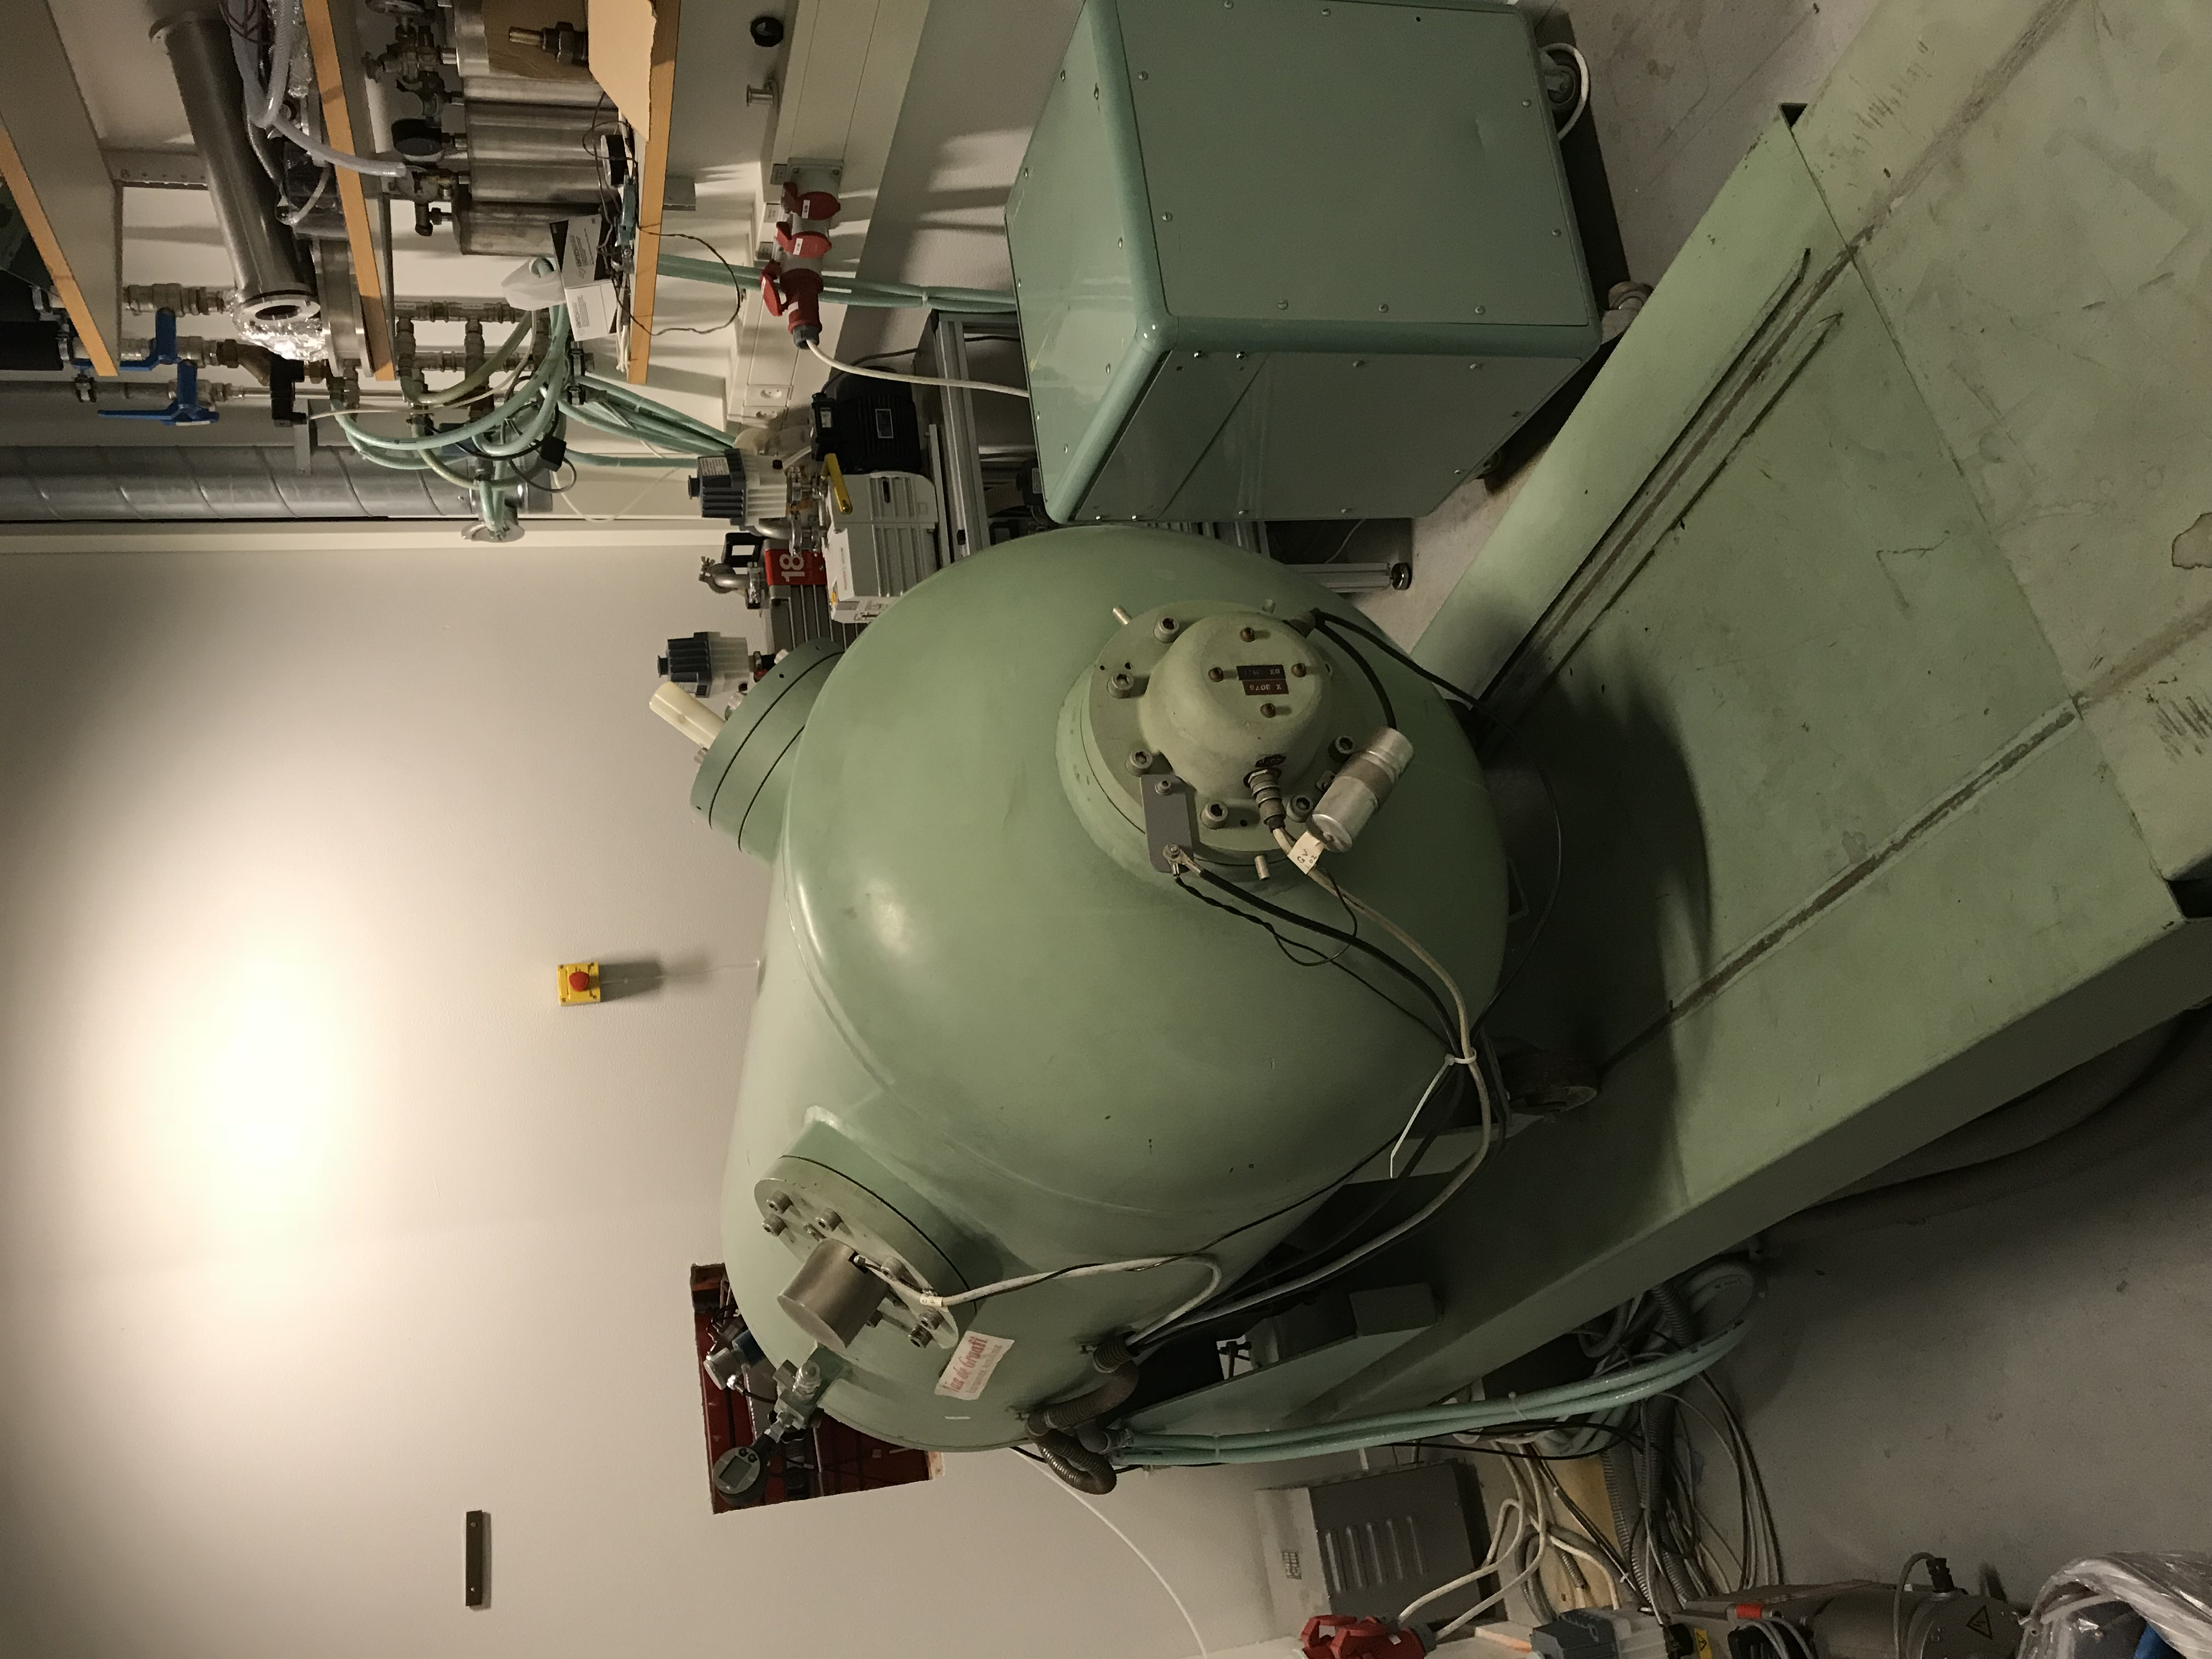
\includegraphics[width=0.5\textwidth]{setup3}
\caption{Experimental setup 3: The single Van-de-Graaf accelerator.}
\label{fig_setup3}
\end{figure}

\subsection{Scattering on atomic nuclei}
The aim of this experiment was to use a particle accelerator to test certain dependencies of Rutherford scattering. Numerically, the Rutherford scattering differential cross section per target atom for any target atom is
\begin{equation}
\frac{d\sigma}{d\Omega} = 1.296 \left( \frac{Z_1 Z_2}{E_\infty [MeV] \, \sin^2 \left(\frac{\theta}{2} \right) }\right)^2\left[\frac{mb}{sr}\right],
\end{equation}
where $\theta$ is the scattering angle, $Z_1$  is the atomic number of the incident particles, $Z_2$ is the atomic number of the target nuclei, and $E_{\infty}$ is their kinetic energy HUSK CITE!%cite 
. 
In order to test these dependencies a relation between the cross section and the count rate (number of scattered particles per time) is found as
\begin{equation}
dN = N \, n_{\text{tar}} \, dx \,d\Omega \, \frac{d\sigma(\theta,\phi)}{d\Omega},
\end{equation}
where $N$ is the number of incoming particles per time, $n_\text{tar}$ is the particle density of the target, $dx$ is the thickness of the target, and $d\Omega$ is the solid angle of the detector.


